\documentclass{beamer}
\usepackage{../../shared/styles/custom}
\usepackage{../../shared/styles/conventions}

\def\checkmark{\tikz\fill[scale=0.4](0,.35) -- (.25,0) -- (1,.7) -- (.25,.15) -- cycle;} 

%\beamerdefaultoverlayspecification{<+->}

\title{Ridge Regression}
\date{\today}
\author{Nipun Batra}
\institute{IIT Gandhinagar}
\begin{document}
  \maketitle

\begin{frame}In $f(x) = c_0 + c_1x + c_2x^2 + \dots$ it is $\max|c_i|$ \\ \bigskip
\end{frame}
  
\begin{frame}\\ \bigskip
\begin{tcolorbox}
\textbf{Objective:}
\begin{align*}
\text{Minimise } & \left(\vy-\mX\vtheta\right)^T\left(\vy-\mX\vtheta\right) \\
\text{s.t. } & \vtheta ^T\vtheta \leq S
\end{align*}
\end{tcolorbox}
\pause
This is equivalent to \vspace{-0.4cm}
$$
\text{Minimise } \left(\vy-\mX\vtheta\right)^T\left(\vy-\mX\vtheta\right) + \delta ^2\vtheta ^T\vtheta
$$
\end{frame}  

\begin{frame}\begin{align*}
\text{Minimise } & \left(\vy-\mX\vtheta\right)^T\left(\vy-\mX\vtheta\right) \\
\text{s.t. } & \vtheta ^T\vtheta \leq S \\
L\left(\vtheta, \mu \right) =& \left(\vy-\mX\vtheta\right)^T\left(\vy-\mX\vtheta\right) + \mu\left(\vtheta^T\vtheta - S\right)
\end{align*}
where, $\mu \geq 0$ (and $\mu = \delta^2$)\bigskip

\pause
\begin{columns}
\begin{column}{0.4\textwidth}
If $\mu = 0$ \\
There is no regularization \\
No effect on constraint
\end{column}
\pause
\begin{column}{0.4\textwidth}
If $\mu\neq 0$ \\
$\implies \vtheta^T\vtheta - S = 0$ 
\end{column}
\end{columns}
\end{frame}

\begin{frame}Are $\theta_{i}$ all zero for high $\mu$?
\end{frame}

\begin{frame}\begin{align*}
\mX^{T}\mX &= \begin{bmatrix}
4 &10\\10&30
\end{bmatrix} \\
(\mX^{T}\mX)^{-1} &= \frac{1}{20} \begin{bmatrix}
30 & -10\\
-10& 4
\end{bmatrix}\\
\mX^{T}\vy &= \begin{bmatrix}
6\\
14
\end{bmatrix}
\end{align*}
\end{frame}

\begin{frame}\begin{align*}
\mX^{T}\mX &= \begin{bmatrix}
4 &10\\10&30
\end{bmatrix} \\
\mX^{T}\mX+\mu \mI &= \begin{bmatrix}
6 &10\\10&32
\end{bmatrix} \\
(\mX^{T}\mX+\mu \mI)^{-1} &= \frac{1}{92} \begin{bmatrix}
32 & -10\\
-10& 6
\end{bmatrix}\\
\mX^{T}\vy &= \begin{bmatrix}
6\\
14
\end{bmatrix}
\end{align*}
\end{frame}

\begin{frame}Another interpretation of ``regularisation''
\end{frame}

\begin{frame}\begin{itemize}
\item Contrast with update equation for unregularised regression:
	\item \(\vtheta=\underbrace{\vtheta}_\text{No Shrinking $\vtheta$} - \alpha(-2 \mX^{\top} \vy+2 \mX^{\top} \mX \vtheta)\)
	
\end{itemize}

\end{frame}

%{
%	\setbeamercolor{background canvas}{bg=}
%	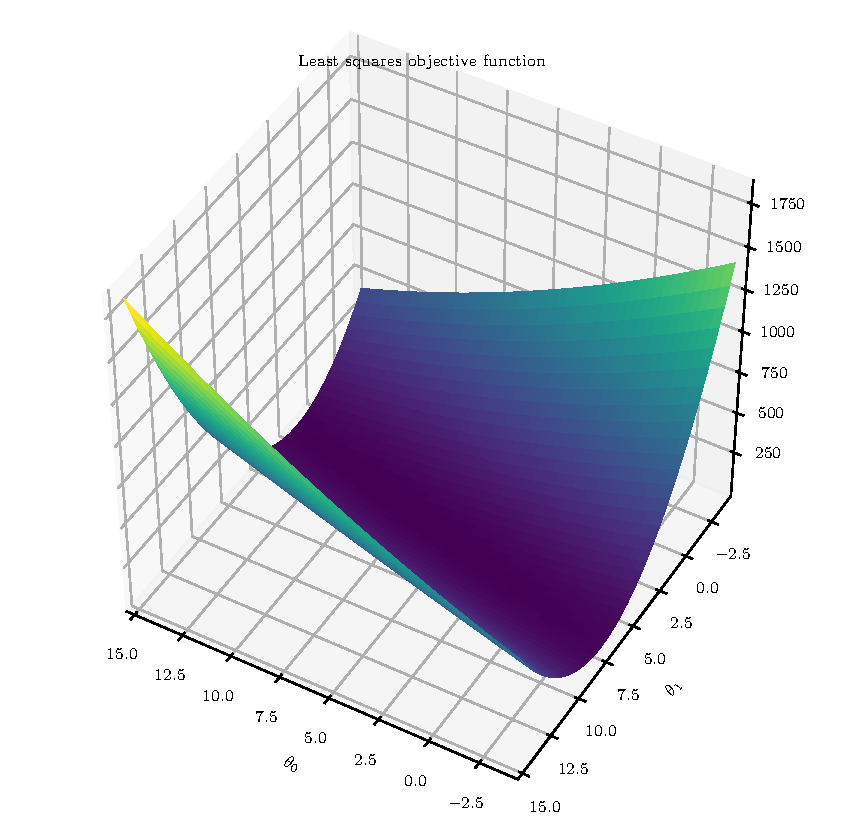
\includepdf[page=-]{ridge-gd.pdf}
%}

\end{document}
